\chapter{Problemfelder innerhalb des Change Managements}
\label{problemfields}

% - erster Hauptteil der Arbeit
% - Herausarbeitung von Veränderungsprozessen und Problemfelder innerhalb der DT

Nach den theoretischen Ausführungen der vorangestellten Kapiteln soll nun inhaltlich auf den ersten Hauptschwerpunkt der vorliegenden Arbeit eingeführt werden. Um in \ref{agilepractices} eine Reihe agiler Methoden hinsichtlich ihrer Anwendbarkeit in Problemfeldern der Digitalen Transformation zu evaluieren, müssen letztere zunächst erarbeitet werden. Dafür soll ein systematisches Literaturreview (\gls{SLR}) von Studien und Fallstudien zum Thema der Digitalen Transformation in Großunternehmen vorgenommen werden. Dadurch hat dieses SLR ebenfalls den Charakter einer \textit{Metastudie}\footnote{Studie, bei der die Ergebnisse verschiedener Untersuchungen bzw. Studien zu einer bestimmten Thematik verglichen, zusammengefasst und nach bestimmten Vorgaben bewertet werden, Definition nach enzyklo.de, online: \url{http://www.enzyklo.de/Begriff/Metastudien}} Aus dieser werden zunächst Veränderungsprozessmuster innerhalb des Transformationsprozesses  zusammengefasst.  Zusätzlich werden auf Grundlage dessen eine Reihe von problematischen Schwerpunkten erarbeitet. Nachfolgend soll zunächst das methodische Vorgehen im aktuellen Kapitel geschildert werden. Es schließt sich eine gesonderte Übersicht der erschlossenen Literatur an, auf dessen Grundlage  die Ergebnisse aufgeführt werden.  Das nachfolgende, erste Literaturreview wird im folgenden durch das Akronym \textit{SLR 1} abgekürzt.

\section{Methodisches Vorgehen}
\label{problemfields:methods}

% - genaue Darstellung über Vorgehen in der SLR + Metastudie
% - Suchmethodik, Keywords, Kriterien, Auswahlprozes ...
% - https://docs.google.com/document/d/1wzYRearLcVTlKJxPp6Mz5U860VoXzkNX7armGeCoxt4/edit

Nachfolgend soll das genaue methodische Vorgehen des ersten systematischen Literaturreviews vorgestellt werden. Vor der eigentlichen Suche nach Fallstudien bzw. relevanter Literatur zum Thema der Digitalen Transformation, wurde eine einheitliche Suchstrategie aufgestellt. Diese wird in \ref{fig:suchstrategie} dargestellt. 

\begin{figure}[H]
	\centering
	\fbox{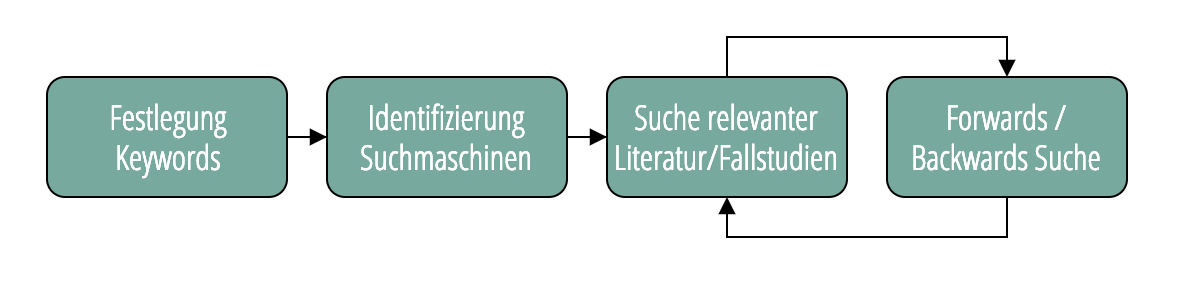
\includegraphics[width=0.8\linewidth]{pics/suchstrategie}}
	\caption[Suchstrategie des SLR]{Suchstrategie des SLR (eigene Darstellung)}
	\label{fig:suchstrategie}
\end{figure}

Wie der Abbildung zu entnehmen wurden zunächst \textit{Keywords} für die  Literatursuche festgelegt. Diese wurden nach einer ersten Probesuche zunehmend angepasst, bis eine zufriedenstellende Ergebnismaske erzielt wurde. Da in der Suche englische  und deutsche Literatur eingeschlossen wurde, wird im folgenden zwischen englischen und deutschen Keywords unterschieden. In \ref{tab:keywordsslr1} werden nachfolgend die \textit{Keyword-Suchketten} aufgeführt, die in sämtlich genutzten Literatursuchmaschinen verwendet wurden. Die Syntax der Suchketten kann dabei  von Suchmaschine zu  Suchmaschine variieren, die Übersicht dient der Allgemeinheit.

\begin{table}[ht]
	\centering
	\caption{Übersicht Keyword-Suchketten SLR 1}
	\begin{tabular}{|p{7cm}|p{7cm}|}
		\hline
		\textbf{Deutsche Keywords}& \textbf{Englische Keywords} \\
		\hline
		digitale+transformation+fallstudie OR digitalisierung+fallstudie   & digital+transformation+case OR digitalization+case \\
		\hline
	\end{tabular}
	\label{tab:keywordsslr1}
\end{table}

Weiter wurden im Vorfeld relevante Literatursuchmaschinen identifiziert. Dabei wurde darauf geachtet, dass überwiegend Suchmaschinen mit Zugang zur technischer sowie wirtschaftlicher Relevant gewählt wurden. Grundsätzlich wurden überwiegend Datenbanken mit vorhandenem Online-Zugang genutzt. \todo{weiter ausführen?} \ref{tab:suchmaschinenslr1} zeigt hierbei  eine Übersicht der genutzten Suchmaschinen mit Angabe der insgesamt gefundenen Literatur.

\begin{table}[ht]
	\centering
	\caption{Übersicht Literatursuchmaschinen SLR 1}
	\begin{tabular}{|p{5cm}|p{7cm}||p{3cm}|}
		\hline
		\textbf{Datenbank/Bibliothek}& \textbf{URL} &  \textbf{Treffer Keywords  (summiert)} \\
		\hline
		IEEE Xplore & \url{https://ieeexplore.ieee.org} & 770 \\
		(Online) - Bibliothek Hochschule Harz & \url{https://opac.lbs-magdeburg.gbv.de/DB=4/LNG=DU} & 6 \\
		(Online) - Bibliothek Technische Universität Berlin  & \url{https://www.ub.tu-berlin.de/literatur-suchen}& 1 \\
		Google Scholar &  \url{https://scholar.google.de}  & 26.800 \\
		Scopus & \url{https://www.scopus.com} & 4.347 \\
		ResearchGate & \url{https://www.researchgate.net} &Keine Angabe vorhanden \footnotemark \\ 
		ACM Digital Library & \url{https://dl.acm.org} & 174.857 \\
		\hline
	\end{tabular}
	\label{tab:suchmaschinenslr1}
\end{table}

\footnotetext{\textit{ResearchGate} bietet keine Funktion zur Angabe der kompletten Treffer-Zahl}

Des Weiteren beinhaltete der vorgenommene Suchprozess eine sogenannte \textit{Forwards - und Backwards-Suche}. Demzufolge wurden mithilfe der bereits gefundenen Fallstudien weitere, zitierte Studien erschlossen (Backwards). Ebenso wurden mithilfe der Suchmaschinen, insoweit die Funktion bereitgestellt wurde, Fallstudien oder Literatur gesucht, die von den gefunden Fallstudien zitiert wurden (Forwards). So konnte eine große Menge von potentiellen Fallstudien  gefunden werden.

Die Angaben zu den Literatur-Treffern in den einzelnen Suchmaschinen zeigt klar, dass eine weitere Filterung vorgenommen werden musste. Dafür wurden ein \textit{Auswahlprozess} definiert, um nur relevante Fallstudien für die folgenden Untersuchungen zu inkludieren. Dieser wird in \ref{fig:auswahlprozess} dargestellt.

\begin{figure}[H]
	\centering
	\fbox{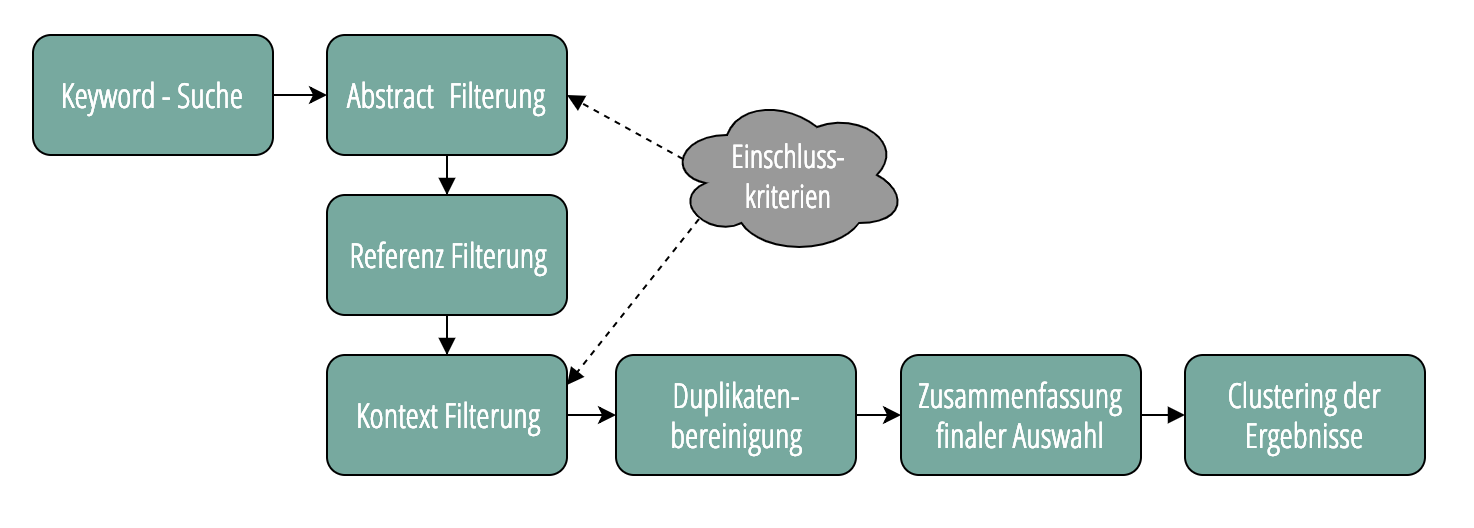
\includegraphics[width=0.8\linewidth]{pics/auswahlprozess}}
	\caption[Auswahlprozess des SLR]{Auswahlprozess des SLR (eigene Darstellung)}
	\label{fig:auswahlprozess}
\end{figure}

Um der großen Menge an Literatur zu begegnen und zu filtern, wurden eine Reihe von Schritten durchgeführt. Wie der \ref{fig:auswahlprozess} zu entnehmen, wurde für die gesamte aus der Keyword-Suche ermittelten Literatur zunächst eine Reihe von \textit{Ein - und Ausschlusskriterien} durchlaufen. Diese bezogen sich zunächst nur auf den Abstract. Sind beispielsweise wesentliche Keywords gar nicht erst wirklich vorhanden, wird die betrachtete Literatur verworfen. Weiterhin wurde überprüft, ob auf eine referenzielle Unverfälschtheit geschlossen werden kann. Dies bedeutet, dass solche Literatur nicht benutzt wird, die augenscheinlich nur eine Kopie einer bereits gefundenen ist; und zwar in dem Zusammenhang, als das sie gegenseitig im Literaturverzeichnis vorkommen. An dieser Stelle sei gesagt, dass dieser Fall sehr vermindert aufgetreten ist. 

Des Weiteren wurden die Ein - und Ausschlusskriterien auf den eigentlichen Inhalt jeder Literatur angewendet. Im Anschluss wurden eine weitere Duplikatenbereinigung durchgeführt. Als Ergebnis dieser Filterungsschritte konnte eine viel kleinere Stückzahl an Fallstudien gewonnen, diese zusammengefasst und geclustert werden.

Im folgenden soll auf die genutzten Ein - und Ausschlusskriterien eingegangen werden. \ref{tab:criteriaslr1} zeigt eine Übersicht der genutzten Kriterien. Grundsätzlich wurde keine Einschränkung in Bezug auf die Nationalität des beschriebenen Unternehmens gemacht. Ebenso gab es keine Beschränkung auf die Branche. Im Bezug auf die \textit{Empirik} wurden nur Fallstudien oder Studien zugelassen. Ebenso mussten alle Objekte eine klare Methodik vorweisen. Demzufolge musste jeweils klar erkenntlich sein, was untersucht wurde und mit welchen wissenschaftlichen Mitteln. Inhaltlich mussten sich die (Fall-)Studien auf die  Implementation einer Digitalen Transformation in einem Großunternehmen drehen. Studien zu KMU wurden  nur dann einbezogen, wenn ein klarer Bezug zu einem größeren Kontext gegeben ist, beispielsweise durch Ausführungen für eine mögliche Skalierung der gefundenen Ergebnisse. Außerdem wurden nur solche Fallstudien inkludiert, die  gesamtorganisationale Schwerpunkt setzen. Dies bedeutet, dass nicht nur auf die Implementation einzelner Technologien, wie beispielsweise \textit{Big Data} eingegangen werden sollte. Ein Bezug auf  das gesamte Unternehmen muss klar erkenntlich sein. Hinsichtlich der gewählten Sprache musste die Literatur auf deutsch oder englisch sein. Das Veröffentlichungsdatum durfte nicht vor dem Jahr 2014 liegen, um eine gewisse Aktualität zu gewährleisten.

\begin{table}[ht]
	\centering
	\caption{Ein - und Ausschlusskriterien SLR 1}
	\begin{tabular}{|p{4cm}|p{8cm}|}
		\hline
		\textbf{Kriterium}& \textbf{Erklärung}  \\
		\hline
		Empirik & Literatur muss eine Fallstudie oder Studie sein \\
		Wissenschaftlichkeit & Methodik der  Fallstudie oder Studie muss klar erkennbar sein \\
		Kontext & inhaltlich Digitale Transformation in Großunternehmen; Mittelständische nur dann, wenn relevant für größeren Kontext \\
		Allgemeinheit & keine Spezifität von einzelnen technischen Implementationen, Gesamtorganisationaler Kontext muss vorhanden sein \\
		Sprache & deutsch oder englisch \\
		Aktualität & ab 2014 - heute  \\
		\hline
	\end{tabular}
	\label{tab:criteriaslr1}
\end{table}

Durch die genutzten Ein - und Ausschlusskriterien konnte die große Menge an Literatur auf eine kleine Gruppe relevanter Fallstudien und Studien im Themenfeld der Digitalen Transformation von Großunternehmen heruntergebrochen werden. Insgesamt konnten \textit{23} Literaturobjekte gefunden werden. Diese beinhalten zusammen rund \textit{200} Fallstudien zu Großunternehmen in verschiedenen Bereichen.

\section{Literaturübersicht}

% - Fallstudien
% - tabellarische Darstellung (https://docs.google.com/document/d/1caHZ-pLGa\_L-TfO4nOh2zZLdAa5nazKaoUZDeDmN90M/edit)
% - Inhaltsangabe jeder Arbeit (Zusammenfassung)

Nachfolgend soll eine kleine Übersicht der gefundenen und gefilterten Literatur gegeben werden, die für die weiteren Untersuchungen verwendet wurden. Eine große Übersicht der  Bücher, wissenschaftlichen Artikeln u.a. findet sich in \ref{tab:overviewliterature1} und \ref{tab:overviewliterature1-2} im Anhang.

Wie im vorangestellten Abschnitt bereits aufgeführt, wurden insgesamt 23 (Fall-)Studien ausgewertet. Nachfolgend soll für jede eine kurze inhaltliche Beschreibung gegeben werden.

\todo{Siehe Tabelle A1 und A2 im Anhang}

\todots

\section{Veränderungsprozessmuster innerhalb der Digitalen Transformation}
\label{problemfields:changepatterns}

% - tabellarische Kreuzmatrix (siehe Link oben)
\todo{Siehe Tabelle A3 im Anhang}

\begin{table}[ht]
	\centering
	\caption{Auswertung Clustering Veränderungsprozessmuster (kurz)}
	\begin{tabular}{|c|c|}
		\hline
		\textbf{Veränderungsprozessmuster}& \textbf{Anzahl Nennungen} \\
		\hline
		Einführung einer Multi-Kanal-Strategie   & 6  \\
		Wechsel vom Offline- zum Online-Vertrieb & 5  \\
		Erschaffung neuer digitaler Produkte     & 12 \\
		Tendenz zur Kundenorientierung           & 16 \\
		Digitalisierung des Geschäftsmodell      & 11 \\
		Digitaler Wissensaufbau im Unternehmen   & 12 \\
		Datengestützte Verbesserungsprozesse     & 5  \\
		Erzeugung eines digitalen Ökosystems     & 7  \\
		Digitalisierung von internen Prozessen   & 7  \\
		Einbindung innovativer Technologien      & 6  \\
		Aufbau technisches Sicherheitskonzept    & 4  \\
		Digitale Neuausrichtung der Organisation & 13 \\
		Innovationsförderung                     & 7  \\
		Kooperation mit externen Treibern        & 5 \\
		\hline
	\end{tabular}
	\label{tab:clusteringvpshort}
\end{table}

\todots

\section{Identifikation von Problemfeldern}

% - tabellarische Kreuzmatrix (siehe Link oben)
\todo{Siehe Tabelle A4 im Anhang}

\begin{table}[ht]
	\centering
	\caption{Auswertung Clustering Problemfelder (kurz)}
	\begin{tabular}{|c|c|}
		\hline
		\textbf{Problemfeld}& \textbf{Anzahl Nennungen} \\
		\hline
		Unternehmensweite Kommunikationsprobleme        & 5  \\
		Festhalten an verfestigten Strukturen           & 7  \\
		Zeit - und Marktdruck                           & 5  \\
		Unterschätzung der Komplexität                  & 4  \\
		Fehlende Kontinuierliche Verbesserungsprozesse  & 7  \\
		Störung durch oberes Management (Top-Down)      & 7  \\
		Konflikte zwischen IT und Business              & 4  \\
		Fehlende frühe Einbeziehung aller Mitarbeiter   & 3  \\
		Sicherheitsprobleme                             & 2  \\
		Fehlende Kundenorientierung                     & 13 \\
		Fehlendes technischen Know-How                  & 10 \\
		Fehlende monetäre Ressourcen                    & 2  \\
		Rechtliche Bestimmungen und Datenschutz         & 5  \\
		Fehlende Transparenz (intern und extern)        & 4  \\
		Fehlende Partnerschaften                        & 6  \\
		Fehlende Innovationskultur                      & 6  \\
		Langsame Entscheidungsprozesse                  & 3  \\
		Unternehmenskulturelle Probleme                 & 8  \\
		Fehlendes Vertrauen, Akzeptanz und Bereitschaft & 9  \\
		Unklare Verantwortlichkeiten                    & 5  \\
		Fehlende digitale Strategie                     & 6 \\
		\hline
	\end{tabular}
	\label{tab:clusteringpfshort}
\end{table}

\todots

\section{Zusammenfassung}


